\section{Hardness of $m$-Robust Correlation Clustering}

\begin{proof}
Consider a simple case - there are just 20 points that naturally form a bipartite ($0$ cost) clustering into 10 points each. Points in the one cluster are similar to each other and dissimlar to points in the other cluster. The edge between point $v_{10}$ in cluster $C_1$ and $v_{20}$ in cluster $C_2$ is changed from a $-$ to a $+$. For this graph, the clustering $\{ C_1,C_2 \}$ is still optimal, now having cost $1$ (since there can be no clusteing of cost $0$). This is shown in Fig.~\ref{fig:1}.

\begin{figure}[ht]
\centering
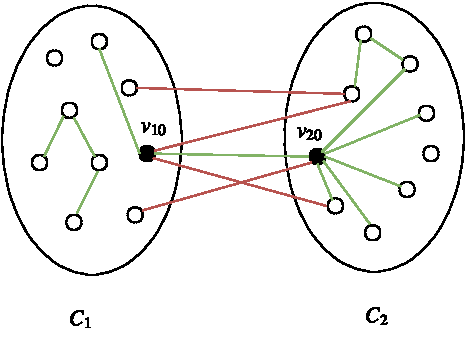
\includegraphics{./img/bipartite.pdf}
\caption{20 points in 2 clusters. $C_1$ and $C_2$ are "natural" clusters}
\label{fig:1}
\end{figure}

Now consider a case where instead of $20 = 2 \times 10$ points, there are $n$ points arranged into $N = 0.1n$ natural clusters with 10 points in each. All 10 points in a cluster are similar to each other and points in different clusters are dissimilar to each other. This is denoted the "natural" clustering which has a cost of $0$ and its components are known as natural clusters.\\

\noindent Now, from each of the $N$ natural clusters, one point is selected and labelled a "bad" point of that cluster. Consider the complete subgraph induced by the bad vertices and swap edges between some pairs of points in this subgraph from $-$ to $+$. This will be the graph we consider in the proof of hardness. Observe that the optimal clustering in this graph is still the natural clustering having cost equal to the total number of $- \to +$ swaps made. This is because points from any two natural clusters cannot be separated with cost lower than $1$ (refer to the paragraph above Fig.~\ref{fig:1}). The natural clustering achieves the least cost for all pairs of clusters - it is $1$ if the edge between bad vertices of the two natural clusters is swapped from $-$ to $+$ and $0$ if not.

\begin{figure}[ht]
\centering
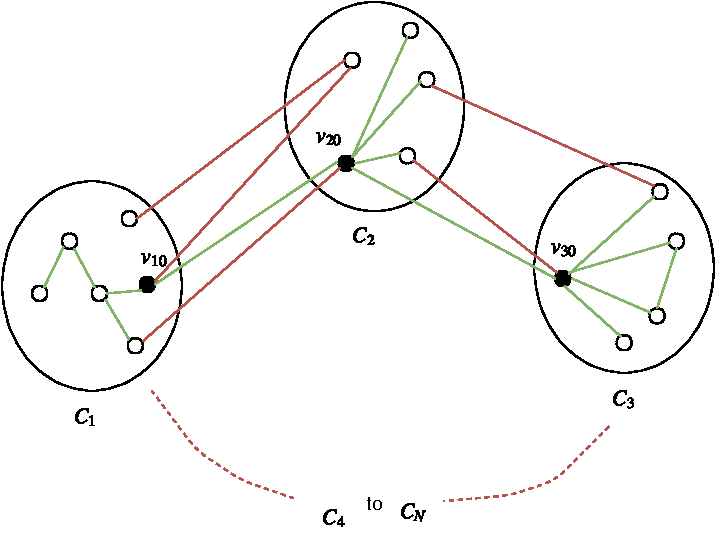
\includegraphics{./img/multipartite.pdf}
\caption{$n$ points with $N$ "natural" clusters - $C_1, C_2, \dots, C_N$}
\label{fig:2}
\end{figure}

In robust correlation clustering, we need to remove $m$ vertices such that the cost of the natural (optimal) clustering on the resultant subgraph is minimized. The choice of these vertices must be from the set of bad vertices, since other vertices do not reduce the clustering cost. Consider an unweighted graph $G'$ defined on the $N$ bad vertices such that if two bad vertices are similar, they have an edge between them and if they are dissimilar, there is no edge between them. This graph captures the $- \to +$ swaps made previously. The goal is to then pick $m$ vertices from this graph such that their removal results in the least number of edges left over. This problem is as hard as vertex cover, since if I can solve it, I can decide if there is a vertex cover of size $m$ (if it is a vertex cover, the number of remaining edges will be $0$. If it is not, the number of edges will be $> 0$). Therefore, it is NP-hard to solve $m$-robust correlation clustering.

\end{proof}